% 1st try cities: https://www.sciencedirect.com/journal/cities
% 
% 2nd choice: Environment and Planning B: Urban Analytics and City Science
% https://journals.sagepub.com/home/EPB

% \documentclass{article}
\documentclass[11pt,journal,compsoc]{IEEEtran}
\usepackage[utf8]{inputenc}
\usepackage{amsmath}
\usepackage{graphicx}
\usepackage{float}
\usepackage{caption}

\begin{document}

\title{Measuring intra-city spatial inequality in the England}

\maketitle
\section{Introduction}

Spatial inequality has received much attention in recent years, with much studies focus on the country or region level inequality. In England, for example, the North-South divide is one of the most well-known phenomenons, with London and the South East consistently outperforming Northern regions on measures of productivity, income, health, and economic opportunity~\cite{martin2016spatially,bambra2018health,carneiro2025not}. Similar macro scale inequalities such as the East-West disparities in Germany~\cite{iammarino2019regional}, and the coastal-inland gradient in China~\cite{wei2009beyond} have been studied as well. In the UK specifically, the Levelling Up agenda introduced by central government in 2022 explicitly acknowledged that regional inequalities had widened over recent decades and set out a framework for narrowing them~\cite{ukgovernment2022levelling,mccann2024levelling}. While these studies have been valuable for highlighting broad structural imbalances, the geographical resolution of regional analysis is inherently coarse. Regional averages, by construction, treat all places within a region as equivalent, and therefore could obscure substantial variation at finer spatial granularities.


In particular, cities are not internally homogeneous, in which neighbourhoods within the same urban area can differ dramatically. There exist some works explored this neighbourhood level inequality, in terms of income, housing conditions, health outcomes, and access to services~\cite{sarkar2024spatial,tammaru2014socio}. \citeauthor{suss2023measuring}~\cite{suss2023measuring} developed a measure of local economic inequality in the UK using housing value data, and \citeauthor{gao2024unpacking}~\cite{gao2024unpacking} examined the inequality in mobility-based exposure. Yet, these existing studies tend to be limited in either geographical (e.g.. Only focus on a few cities) or thematic scope (only focus on limited dimensions of inequalities). What remains missing is a comprehensive, England-wide analysis that systematically compares city-level inequality.


In this paper, we adopt the Index of Multiple Deprivation (IMD) published by Ministry of Housing, Communities and Local Government (MHCLG) for such as analysis. IMD combines seven weighted domains, including income, employment, education, health, crime, barriers to housing and services, and the living environment, into a single relative deprivation score for each Lower Layer Super Output Area (LSOA) in England, as shown in Figure 1~\cite{mcclennan2025english}. There are 33,755 LOSAs in England, each containing an average population of roughly 1,500 residents, and making IMD to be one of the most spatially granular official deprivation measures available (ref to add). IMD has been widely used in research across public health~\cite{marmot2020health}, education~\cite{gorard2016cautionary}, and urban policy~\cite{norman2016changing}, and has informed official resource allocation decisions. The most recent release, IMD 2025, updates the established methodology of IMD 2019 with new input data, providing a current small-area deprivation snapshot well-suited to our city-level inequality analysis.

\begin{figure}[t]
    \centering
    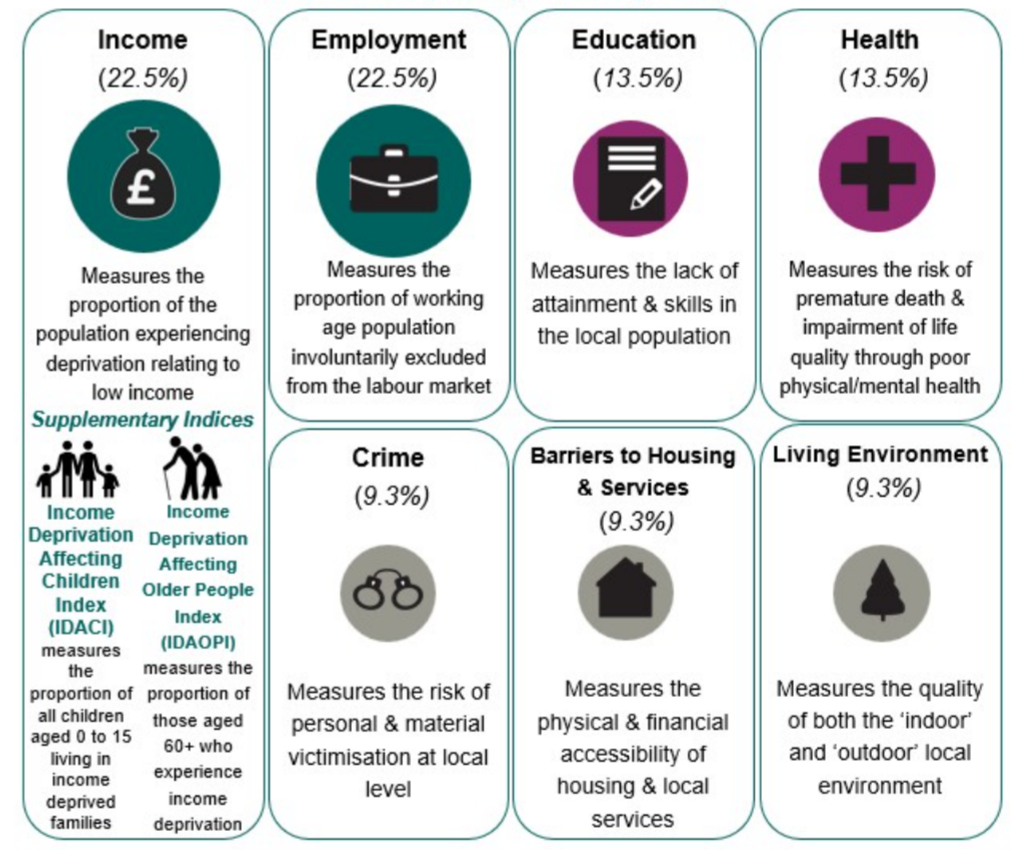
\includegraphics[width=1.0\columnwidth]{figure1.png}
    \caption{The seven domains of deprivation that combine to create the Index of Multiple Deprivation (IMD25)}
    \label{fig:fig1}
\end{figure}

Using the IMD to measure intra-city inequality, however, presents two key challenges. The first is aggregation. The IMD is designed as a relative ranking of small areas, not as a direct measure of inequality within cities. Moving from LSOA-level observations to city-level summaries requires linking each LSOA to a Local Authority District (LAD) and then mapping each LAD to an analytical city unit. Because LSOAs vary in population size, population weighting is needed to ensure that each resident contributes equally to the city summary rather than each spatial unit receiving equal influence. The second challenge is spatial structure. The standard Gini coefficient can capture the overall spread of deprivation scores within a city, but it is locationally invariant, in which it cannot distinguish a city where deprived areas are scattered throughout the urban fabric from one where they are sharply segregated into contiguous clusters~\cite{arbia2001role}. The spatial decomposition of the Gini~\cite{rey2013spatial,panzera2020measuring} addresses this by partitioning total inequality into a spatially structured component and a non-spatial component, quantifying the degree to which deprivation clusters geographically.


This paper addresses these challenges by providing a systematic analysis of intra-city inequality across 54 English cities using IMD 2025, covering a total of X LSOAs and approximately X million residents. We construct five population-weighted indicators organised into two dimensions as follows. (1) Deprivation level: (a) weighted mean IMD score, (b) share of the city population in the most deprived national decile, and (c) share in the most deprived two deciles) and (2) internal inequality: (a) a population-weighted Gini coefficient, and (b) a spatial Gini measuring the share of inequality attributable to geographical clustering), and compare the correlation between them in different cities. The contributions are threefold. First, we provide an England-wide city-level analysis of internal deprivation inequality, filling the space between broad regional overviews and single-city case studies. Second, we apply a spatial Gini decomposition at the city scale, enabling direct comparison of the degree of spatial segregation across the English urban system. Third, we identify distinct city typologies where deprivation level and internal inequality diverge, providing evidence for more targeted urban policy.


Our results shows that, generally the deprivation level of a city and its intra-city inequality are positively correlated (correlation coefficient XX). But cities with similar average deprivation scores can differ substantially in how unevenly that deprivation is distributed internally. For instance, St Albans has a low-deprivation but high-inequality, while Bradford combines high deprivation with above-average inequality. London, despite its size and overall deprivation, does not sit in the highest-inequality quadrant. In terms of spatial distribution of inequality within cities, a large share of the observed inequality appears spatially clustered, in which deprivation cluster across contiguous neighbourhoods rather than being locally mixed, but the degree of spatial segregation varies considerably across cities. These findings demonstrate that aggregated city-level deprivation summaries alone are insufficient for understanding the internal geography of disadvantage, and that distinguishing between the level, dispersion, and spatial configuration of deprivation provides a richer evidence base for urban policy.


The rest of the paper is organised as follows. Section 2 reviews the relevant literature. Section 3 describes the data sources and methodology. Section 4 presents the results. Section 5 discusses the implications and limitations of the study. Section 6 concludes the paper and outlines directions for future work.

\section{Literature Review}
\subsection{Intra-city spatial inequality}

Research on spatial inequality has traditionally focused on differences across countries and regions. In the UK, this is reflected in longstanding debates on the North--South divide and broader patterns of uneven development, with persistent disparities in productivity, employment, income, and health ~\cite{martin2016spatially,bambra2014north,mccann2016uk}. Comparable macro-spatial inequalities have been documented elsewhere, including East--West divides in Germany and coastal--inland divergence in China ~\cite{iammarino2019regional,wei2009beyond}. This body of work has been influential in demonstrating that inequality is spatially structured, but its coarse geographical scale necessarily obscures variation within cities. More recent reviews emphasise that cities are not merely passive containers of inequality but active systems in which spatial form, infrastructure, and access jointly shape unequal outcomes within urban space ~\cite{sarkar2024spatial}.

Cities are not internally homogeneous socio-spatial units. Neighbourhoods within the same urban area can differ markedly in deprivation, housing quality, access to services, and health outcomes. The neighbourhood-effects literature shows that local context shapes individual trajectories through mechanisms such as peer interaction, institutional access, and information flows ~\cite{ellen1997does,galster2011mechanism,tammaru2014socio}. In parallel, the segregation literature demonstrates that the spatial separation of social groups is not merely descriptive but constitutive of inequality, as uneven access to opportunities becomes embedded in residential patterns ~\cite{massey1988dimensions,tammaru2014socio}. From this perspective, intra-city inequality is not a residual of regional disparities but a distinct process operating at the urban scale.

Recent work has reinforced this shift in focus. Socio-economic segregation has been identified as a defining feature of contemporary European cities ~\cite{tammaru2014socio}, while neighbourhood inequality has been shown to persist through durable social and institutional mechanisms ~\cite{sampson2012great}. Rising income inequality is also associated with increasing spatial segregation ~\cite{reardon2011income}, suggesting that distributional and spatial processes are closely intertwined. More broadly, urban theory has long treated cities as key arenas through which inequality is produced and reproduced ~\cite{massey1974social,fainstein2014just,soja2013seeking,florida2017new}.

The local scale is not only empirically relevant but also theoretically salient. Relative deprivation is evaluated against proximate others ~\cite{runciman1966relative,smith2012relative}, and empirical evidence shows that well-being responds to local income comparisons ~\cite{luttmer2005neighbors}. Recent UK-based work similarly highlights the perceptual salience of neighbourhood-scale inequality ~\cite{suss2023measuring}, while deprivation may also be experienced through daily activity spaces rather than residential location alone ~\cite{comber2022dynamic}.

In the UK context, empirical studies of intra-urban inequality have often focused on specific dimensions such as housing markets, health disparities, or education outcomes, frequently at the level of individual cities or metropolitan regions~\cite{bambra2014north,comber2022dynamic,suss2023measuring}. While these studies provide valuable insights into localised processes of disadvantage, they are typically limited in geographical coverage and do not support systematic comparison across cities within a unified analytical framework.

\subsection{Spatial measures of inequality}

The Gini coefficient remains one of the most widely used summary measures of inequality due to its simplicity and comparability ~\cite{cowell2011measuring}. In the context of urban analysis, it provides a convenient scalar indicator of how unevenly a variable is distributed across neighbourhoods within a city. However, the conventional Gini coefficient is fundamentally aspatial, meaning that identical distributions can yield identical Gini values regardless of their spatial configuration.

This limitation is analytically significant. A city in which deprivation is concentrated in contiguous clusters differs fundamentally from one in which high- and low-deprivation neighbourhoods are locally interspersed, yet both may exhibit the same level of overall inequality. As a result, aspatial measures capture dispersion but not spatial structure. This distinction has long been recognised in the spatial inequality literature. Arbia~\cite{arbia2001role} separates the distribution of values from their spatial arrangement, while Rey and Janikas~\cite{rey2005regional} argue that inequality and spatial dependence should be analysed jointly. Bickenbach and Bode~\cite{bickenbach2008disproportionality} similarly demonstrate that conventional concentration measures are not well suited to capturing spatial phenomena.

Methodological responses have therefore focused on extending the Gini coefficient to incorporate spatial relationships. Rey and Smith~\cite{rey2013spatial} propose a spatial decomposition that distinguishes inequality arising between neighbouring and non-neighbouring observations. Building on this, Panzera and Postiglione~\cite{panzera2020measuring} develop a Gini-correlation framework that quantifies the share of total inequality attributable to spatial clustering. Related approaches have also been applied in segregation analysis ~\cite{turk2023introducing}. These contributions establish that overall dispersion and spatial configuration are analytically separable dimensions and should not be collapsed into a single summary statistic. Compared with alternative spatial measures such as Moran's I, which captures spatial autocorrelation but not inequality magnitude, or segregation indices that are typically defined for discrete groups, the spatial Gini framework is particularly suited to continuous deprivation measures. It allows the joint assessment of dispersion and spatial arrangement within a single, comparable metric, making it well aligned with the objectives of intra-city inequality analysis.

Population weighting is a critical component of this framework. Small-area spatial units differ substantially in population size, and unweighted measures assign equal importance to areas rather than individuals. The theoretical basis for weighted inequality measurement is well established ~\cite{mookherjee1982decomposition}, and its relevance to spatial analysis has been emphasised in recent work~\cite{panzera2020measuring}. For LSOA-based analysis, this implies that inequality should be measured on a person-weighted basis to reflect the distribution of deprivation experienced by residents rather than the distribution of values across arbitrary spatial units.

Despite these advances, an important gap remains. Much of the existing literature focuses on income, GDP, or other single-dimensional indicators and is often applied at regional or inter-municipal scales. Applications at the intra-city level are comparatively limited, and even fewer studies combine population weighting with spatial decomposition in a way that enables systematic comparison across cities. In particular, the integration of spatial inequality measures with multidimensional deprivation indicators at the fine neighbourhood scale remains underdeveloped.

\subsection{IMD and deprivation}

The Index of Multiple Deprivation (IMD) provides a suitable empirical basis for analysing intra-city inequality. The English Indices of Deprivation 2025 measure relative deprivation across 33,755 Lower-layer Super Output Areas (LSOAs), combining seven domains---income, employment, education, health, crime, barriers to housing and services, and living environment---into a composite indicator ~\cite{mcclennan2025english}. Its multidimensional structure and fine spatial resolution make it particularly well suited to capturing variation in deprivation within cities.

The conceptual foundation of deprivation lies in Townsend's~\cite{townsend1987deprivation} definition of relative disadvantage, which emphasises observable exclusion from the living conditions and activities considered normal in society. This framework underpins the development of multidimensional measures that extend beyond income to capture broader forms of social and material disadvantage. In England, IMD has become the standard approach for identifying neighbourhood-level deprivation ~\cite{mclennan2019english} and is widely used in both research and policy contexts. Its consistency, official status, and policy relevance make it a robust basis for comparative urban analysis.

Existing research using IMD, however, remains fragmented in its analytical focus. A large share of the literature employs IMD descriptively to identify deprived areas or explain variation in outcomes such as health and educational attainment. Other work extends deprivation beyond the residential neighbourhood, for example, by incorporating activity spaces to capture exposure across the city ~\cite{comber2022dynamic}. Related work further shows that inequality within cities is also reflected in mobility patterns and access to activity spaces, highlighting how exposure to opportunities varies across socio-economic groups beyond residential location ~\cite{gao2024unpacking}. Alternative approaches use locally salient indicators, such as housing values, to measure neighbourhood inequality more directly ~\cite{suss2023measuring}, but these often lack comparability across cities.

As a result, the literature has developed along parallel rather than integrated lines. IMD-based studies tend to emphasise deprivation levels rather than internal inequality. Methodological work on spatial inequality tends to focus on economic indicators rather than multidimensional deprivation. UK-based studies of neighbourhood inequality are often limited to specific cities or indicators, reducing their comparability.

This fragmentation leaves a clear empirical gap. There is limited evidence on how multidimensional deprivation is distributed within cities, how unequal these distributions are across neighbourhoods, and to what extent inequality is spatially structured rather than locally mixed. This also implies that city-level deprivation cannot be treated as a single scalar condition: average deprivation, exposure to extreme deprivation, internal inequality, and spatial configuration may diverge substantially across cities. This highlights the need for a framework that integrates multidimensional deprivation with population-weighted and spatially decomposed measures of inequality across cities, which this study seeks to provide.

\section{Data and Research Design}

\subsection{Data Sources}

This study draws on the Index of Multiple Deprivation 2025 (IMD 2025) as its sole data source. Published by the UK government in 2025, IMD 2025 is the most recent official measure of small-area deprivation in England. Its domain structure and methodological framework are consistent with the previous release, IMD 2019, making it a reliable basis for cross-city comparison.

IMD 2025 is constructed at the level of Lower-layer Super Output Areas (LSOAs), the standard small-area geographic units in England's national statistical system, each covering approximately 1,500 residents on average. This resolution is fine enough to preserve the neighbourhood-level variation within cities that lies at the heart of this study's analytical interest. The index also provides a consistent relative deprivation measure across all of England, which allows meaningful comparison across the 54 cities in the sample. 

\subsection{Geographic Units and Spatial Aggregation}

The analysis operates across three spatial levels, each serving a distinct role in the aggregation framework.

LSOAs form the observational unit of the analysis. All IMD 2025 domain scores and composite rankings are recorded at this scale, making them the primary carrier of deprivation information in this study.

Local Authority Districts (LADs) serve as the intermediate linking geography rather than the substantive unit of analysis. Each LAD corresponds to the jurisdiction of a single local government authority, and its boundaries nest directly and consistently above the LSOA level. This nesting relationship is what allows LSOA-level deprivation data to be assembled into city-level indicators in a systematic and traceable way.

Cities are the final analytical unit and the scale at which the research questions are answered. City status in England is an honorary designation and does not correspond to any standardised statistical boundary suitable for data aggregation. This study therefore uses each city's corresponding LAD boundary as an operational proxy. This approach is justified on two grounds: LAD boundaries align directly with the LSOA nesting structure, enabling clean data aggregation, and they broadly correspond to the functional extent of cities as residential and labour market units. Applying the same operationalisation to all cities also ensures comparability across the sample.

England's official list contains 55 cities. Because London and Westminster share a single LAD boundary, they are merged into one analytical unit, yielding a final sample of 54 cities.
\section{Methodology}

Data processing begins at the LSOA level. IMD 2025 scores are merged with resident population counts for each LSOA, after which each LSOA is linked to its parent LAD using the official ONS geographic lookup file. The constituent LSOAs for each of the 54 analytical cities are then selected according to the city-to-LAD correspondence established in Section 3. The attribute data are subsequently joined to the 2021 England LSOA boundary file and reprojected to the British National Grid (EPSG:27700) in preparation for spatial weight matrix construction. On this basis, population weights are applied to all LSOAs within each city, and indicators across three dimensions, namely overall deprivation level, extreme deprivation exposure, and internal inequality, are computed. The measurement framework for each dimension is described in the sections that follow.

\subsection{The Necessity of Population Weighting}

 Equal weighting assigns the same importance to every LSOA regardless of how many people live there, which means the resulting city-level summary answers the question of what deprivation looks like for the average spatial unit rather than for the average resident. In practice, LSOAs with unusually small populations or irregular boundaries exert disproportionate influence on city means, so two cities whose residents have similar lived experiences may appear statistically different simply because their LSOA partitions differ. This introduces a systematic bias into cross-city comparisons that has nothing to do with underlying inequality.

This problem is well recognised in the spatial inequality literature. Panzera and Postiglione~\cite{panzera2020measuring}, in developing a spatial decomposition of regional inequality, argue explicitly that regional per capita income must be weighted by population share to reflect the number of people that figure represents, and they build their Gini-based framework on this principle ~\cite{mookherjee1982decomposition}. This study applies the same logic at the intra-city level. Each LSOA $i$ is assigned a population weight

$$\pi_i = \frac{p_i}{\sum_i p_i}$$

where $p_i$ is the resident population of LSOA $i$ and $\sum_i \pi_i = 1$. Under this scheme, every resident contributes equally to the city-level summary, neighbourhoods with larger populations receive correspondingly greater influence, and the resulting indicators carry a direct person-based interpretation that is meaningful for policy discussions about resource allocation.

\subsection{Construction of the Five Indicators}

This study constructs five city-level indicators spanning three analytical dimensions, together forming a framework for characterising intra-city deprivation patterns.

The first dimension captures the overall level of deprivation through the population-weighted mean IMD score, defined as

$$\bar{IMD}^{*}_{c} = \sum_{i \in c} \pi_i \cdot IMD_i = \frac{\sum_{i \in c} p_i \cdot IMD_i}{\sum_{i \in c} p_i}$$

This indicator summarises the average deprivation environment experienced by residents of city $c$ and serves as the baseline for cross-city comparisons of overall poverty levels.

The second dimension measures exposure to extreme deprivation. The indicator $p_{decile1}$ is defined as the share of a city's population living in LSOAs that fall within the most deprived $10\%$ nationally (national deprivation decile 1):

$$p_{decile1,c} = \frac{\sum_{i \in c} p_i \cdot \mathbf{1}[\text{decile}_i = 1]}{\sum_{i \in c} p_i}$$

A companion indicator, $p_{decile1\_2}$, extends the threshold to the most deprived $20\%$ nationally, providing a broader measure of severe deprivation exposure. These two indicators complement the mean score: whereas the mean is sensitive to the shape of the full distribution, the exposure indicators focus on the left tail and directly quantify the scale of the population living in the most deprived neighbourhoods.

The third dimension addresses internal inequality in both its overall magnitude and its spatial structure, and it forms the methodological core of this study. The theoretical foundations of the two indicators in this dimension are discussed in detail in Section 4.4.

The first indicator is the population-weighted Gini coefficient $G^*$, which measures the overall dispersion of IMD scores across LSOAs within a city under population weighting. Following Lerman and Yitzhaki (1989), a weighted midpoint cumulative distribution function is defined for each LSOA $i$ as

$$F^*_Y(y_i) = \sum_{j=0}^{i-1} \pi_j + \frac{\pi_i}{2}, \quad i = 1, 2, \ldots, n$$

where the $y_i$ are sorted in ascending order and $\pi_0 = 0$. The weighted Gini coefficient is then given by (Panzera \& Postiglione, 2020, Eq.~11)

$$G^* = \frac{2 \cdot \text{Cov}_w\!\left(y,\, F^*_Y(y)\right)}{\mu^*_y}$$

where the weighted covariance is

$$\text{Cov}_w\!\left(y,\, F^*_Y(y)\right) = \sum_i \pi_i \left(y_i - \mu^*_y\right)\left(F^*_Y(y_i) - \bar{F}^*\right)$$

with $\mu^*_y = \sum_i \pi_i y_i$ denoting the population-weighted mean and $\bar{F}^* = \sum_i \pi_i F^*_Y(y_i)$. A higher $G^*$ indicates greater disparity in deprivation across the neighbourhoods within a city.

The second indicator is the population-weighted spatial Gini coefficient $G^*_S$, which extends $G^*$ by introducing a spatial dimension designed to isolate the component of inequality driven by neighbourhood spatial dependence (Panzera \& Postiglione, 2020, Eq.~12). The construction replaces the rank ordering of $y_i$ in the $G^*$ formula with the rank ordering of the spatially lagged variable $Wy_i$, a procedure known as spatial reranking (Dawkins, 2007). This identifies how much of the city's internal inequality stems from high-deprivation neighbourhoods being geographically adjacent to other high-deprivation neighbourhoods:

$$G^*_S = \frac{2 \cdot \text{Cov}_w\!\left(y,\, F^*_{WY}(Wy)\right)}{\mu^*_y}$$

where $F^*_{WY}(Wy_i)$ is the weighted midpoint cumulative distribution function evaluated on the spatially lagged values $Wy_i$, computed by the same procedure as $F^*_Y(y_i)$. It is important to note that spatial reranking affects only the rank ordering used in the covariance; the variable being explained in the numerator remains the original deprivation score $y_i$ rather than the spatial lag $Wy_i$. A higher $G^*_S$ indicates that deprivation within a city is more strongly concentrated into contiguous clusters, reflecting a higher degree of spatial segregation.

The five indicators are designed to be read jointly. The mean score $\bar{IMD}^*$ and the decile exposure shares together answer how deprived a city is overall and how many residents live in its most deprived neighbourhoods. $G^*$ then answers how unequally that deprivation is distributed across neighbourhoods within the city. $G^*_S$ goes further and asks whether that inequality takes the form of spatial clustering rather than local mixing. The separability of $G^*$ and $G^*_S$ is particularly important: two cities with identical $G^*$ values can differ sharply in $G^*_S$, with one exhibiting highly spatialised inequality concentrated in distinct deprived zones and the other showing deprivation that is locally mixed across neighbouring areas. These two configurations carry very different policy implications despite producing the same overall Gini coefficient.

\subsection{Spatial Decomposition Framework}

\subsubsection{The Anonymity Limitation of the Standard Gini Coefficient}

Although $G^*$ accurately measures the overall dispersion of deprivation scores within a city, it satisfies the anonymity axiom, meaning it is entirely insensitive to the spatial arrangement of observations~\cite{bickenbach2008disproportionality}. Holding the distribution of LSOA deprivation scores constant, $G^*$ takes the same value regardless of whether high-deprivation and low-deprivation neighbourhoods are geographically adjacent, forming concentrated clusters, or spatially interleaved in a locally mixed pattern. These two configurations differ substantially in terms of residential segregation, geographic inequality of opportunity, and the appropriate policy response, so it is important to distinguish between them at the measurement level. Panzera and Postiglione~\cite{panzera2020measuring} characterise this as the permutational invariance of conventional inequality measures: different spatial arrangements of the same distribution produce identical inequality statistics~\cite{rey2005regional}, which means $G^*$ alone cannot distinguish between large inequality that is spatially dispersed and large inequality that is spatially concentrated.

\subsubsection{Spatial Decomposition via the Gini Correlation Measure}

To incorporate the spatial dimension into inequality measurement, this study adopts the Gini correlation-based spatial decomposition introduced by Panzera and Postiglione~\cite{panzera2020measuring}, which in turn builds on the Gini correlation measure of Schechtman and Yitzhaki (1987). The central intuition is that if deprivation within a city exhibits strong positive spatial autocorrelation, the deprivation score $y_i$ of a given LSOA should correlate positively with the population-weighted average deprivation score of its neighbours, that is, the spatial lag $Wy_i$. If deprivation is distributed close to randomly in space, this association approaches zero.

On this basis, the population-weighted Gini coefficient admits a decomposition into spatial and non-spatial components (Panzera \& Postiglione, 2020, Eq.~14):

$$G^* = G^*_S + G^*_{NS}$$

where $G^*_{NS} = G^* - G^*_S$ and $0 \leq G^*_{NS} \leq 2G^*$ captures the residual inequality that cannot be attributed to the observed pattern of spatial dependence. The spatial share $\gamma^*$ is then defined as (Panzera \& Postiglione, 2020, Eq.~13)

$$\gamma^* = \frac{G^*_S}{G^*} = \frac{\text{Cov}_w\!\left(y,\, F^*_{WY}(Wy)\right)}{\text{Cov}_w\!\left(y,\, F^*_Y(y)\right)}$$
where $F^*_{WY}$ is ...

The index $\gamma^*$ ranges over $[-1, 1]$ (Schechtman \& Yitzhaki, 1999) and can be interpreted directly as the proportion of total intra-city inequality explained by spatial clustering. When $\gamma^* = 1$, the ranking of $Wy$ is identical to that of $y$, so all inequality is driven by spatial concentration. When $\gamma^* = 0$, $y$ and $Wy$ are uncorrelated and inequality is entirely non-spatial in origin. Positive values of $\gamma^*$ reflect positive spatial autocorrelation, indicating that high-deprivation neighbourhoods tend to be located next to other high-deprivation neighbourhoods, and $\gamma^*$ therefore serves as a direct measure of spatial segregation.

\subsubsection{Construction of the Spatial Weight Matrix}

Computing the spatial lag $Wy_i$ requires an explicit definition of the neighbourhood relationship for each LSOA. This study constructs the spatial weight matrix $W$ using the $k$-nearest neighbours (kNN) criterion. For each analytical city, a separate kNN weight matrix is built from the centroid coordinates of the LSOA polygons, projected onto the British National Grid (EPSG:27700), and row-standardised so that $Wy_i$ equals the simple average of the deprivation scores of the $k$ nearest LSOAs. Constructing the weight matrix independently for each city ensures that neighbourhood relationships are confined within city boundaries, preventing cross-city spatial spillovers from contaminating the intra-city inequality estimates. This approach is consistent with the kNN specification used in the empirical application of Panzera and Postiglione~\cite{panzera2020measuring}.

\subsubsection{Primary Specification and Robustness Checks}

The primary specification sets $k = 5$, following the default used in the empirical application of Panzera and Postiglione~\cite{panzera2020measuring}. As a robustness check, $G^*$, $G^*_S$, and $\gamma^*$ are also computed independently for all 54 cities under $k \in \{5, 7, 10\}$. If city rankings are highly consistent across specifications, with cross-specification correlations of $\gamma^*$ close to one and differences in point estimates uniformly small, this provides evidence that the decomposition results are not sensitive to the particular choice of $k$.

\section{Results and Discussion}

\subsection{Deprivation Level and Intra-city Inequality Are Empirically Separable Dimensions}

A city's overall poverty level and the degree of deprivation inequality across its neighbourhoods are two empirically independent dimensions. This finding directly challenges a widely held assumption in policy discussion, namely that highly deprived cities necessarily exhibit high internal inequality.

Plotting the 54 cities by mean deprivation score and population-weighted Gini coefficient $G^*$ reveals a loose positive association, but one with limited explanatory power (Figure 2). All four quadrants of the scatter plot contain a substantial number of cities, and roughly one third of cities fall in quadrants that contradict the intuitive expectation. The two most instructive contrasting cases are St Albans, with a mean deprivation score of approximately 8, among the lowest in the sample, yet a $G^*$ of around 0.46, the highest of all 54 cities, and Manchester, with a mean score of approximately 38, the highest overall poverty level in the sample, yet a $G^*$ of only around 0.27, below the sample median. The two cities differ by more than 30 units on the deprivation scale but are ranked in opposite order on internal inequality.

\begin{figure}[t]
    \centering
    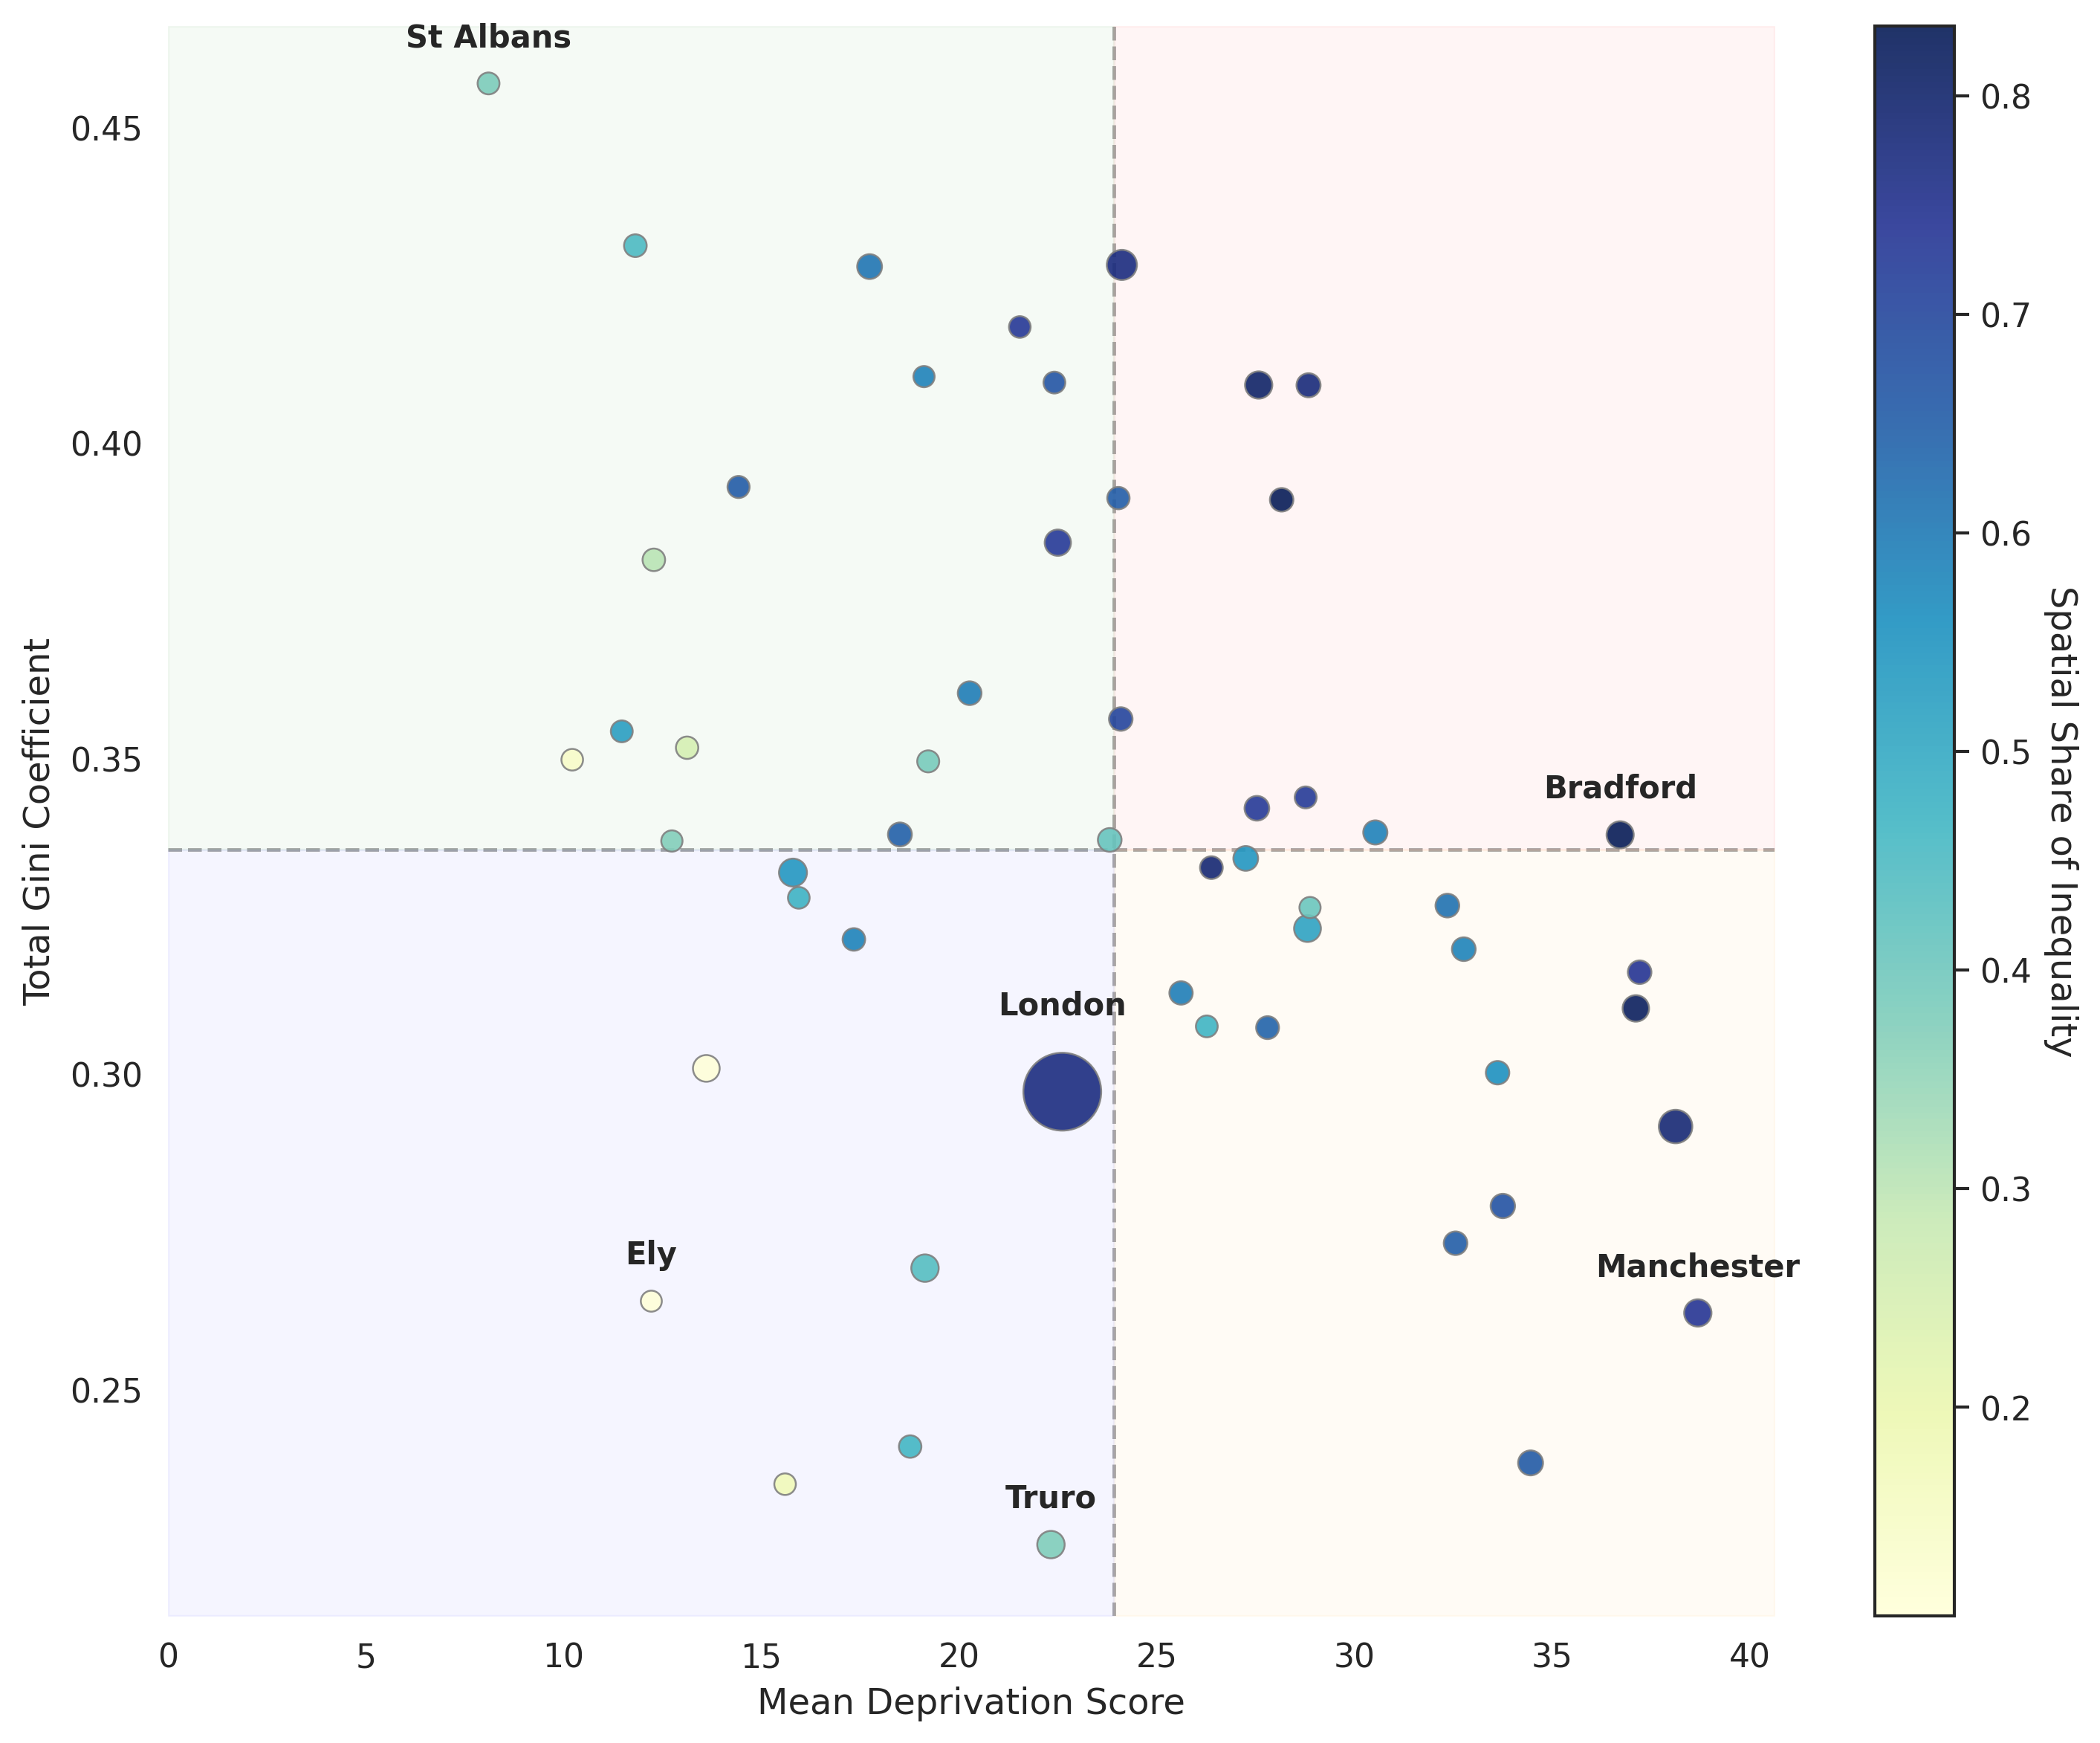
\includegraphics[width=1.0\columnwidth]{figure2.png}
    \caption{Urban Pathology Matrix: Deprivation vs Inequality}
    \label{fig:fig1}
\end{figure}
%a table listing all city result

This is not a peculiarity of St Albans or Manchester but reflects a broader structural fact: a highly deprived city can be internally homogeneous, while a relatively affluent city can be highly polarised within. The two dimensions capture different aspects of a city's internal structure and are not interchangeable either statistically or in terms of policy implications. An analysis that focuses solely on mean deprivation will systematically overlook the kind of internal risk that St Albans represents, while one that focuses solely on internal inequality will understate the aggregate poverty pressure that characterises Manchester.

Cities such as Bradford do rank highly on both dimensions, which confirms that a positive tendency exists between the two. But the existence of that tendency makes cities that deviate from it more important to identify, since their configurations cannot be captured by any single-dimensional analysis.

The radar chart profiles of six extreme cities (Figure 3) reinforce this point. Manchester extends to the outer ring on the average deprivation and extreme deprivation rate axes but shows a relatively compressed total inequality axis. St Albans presents the mirror image: its deprivation axes collapse toward the centre while the inequality axis extends prominently outward. The near-symmetry of the two profiles provides a visual representation of the separability between the two dimensions.

\begin{figure*}[t]
    \centering
    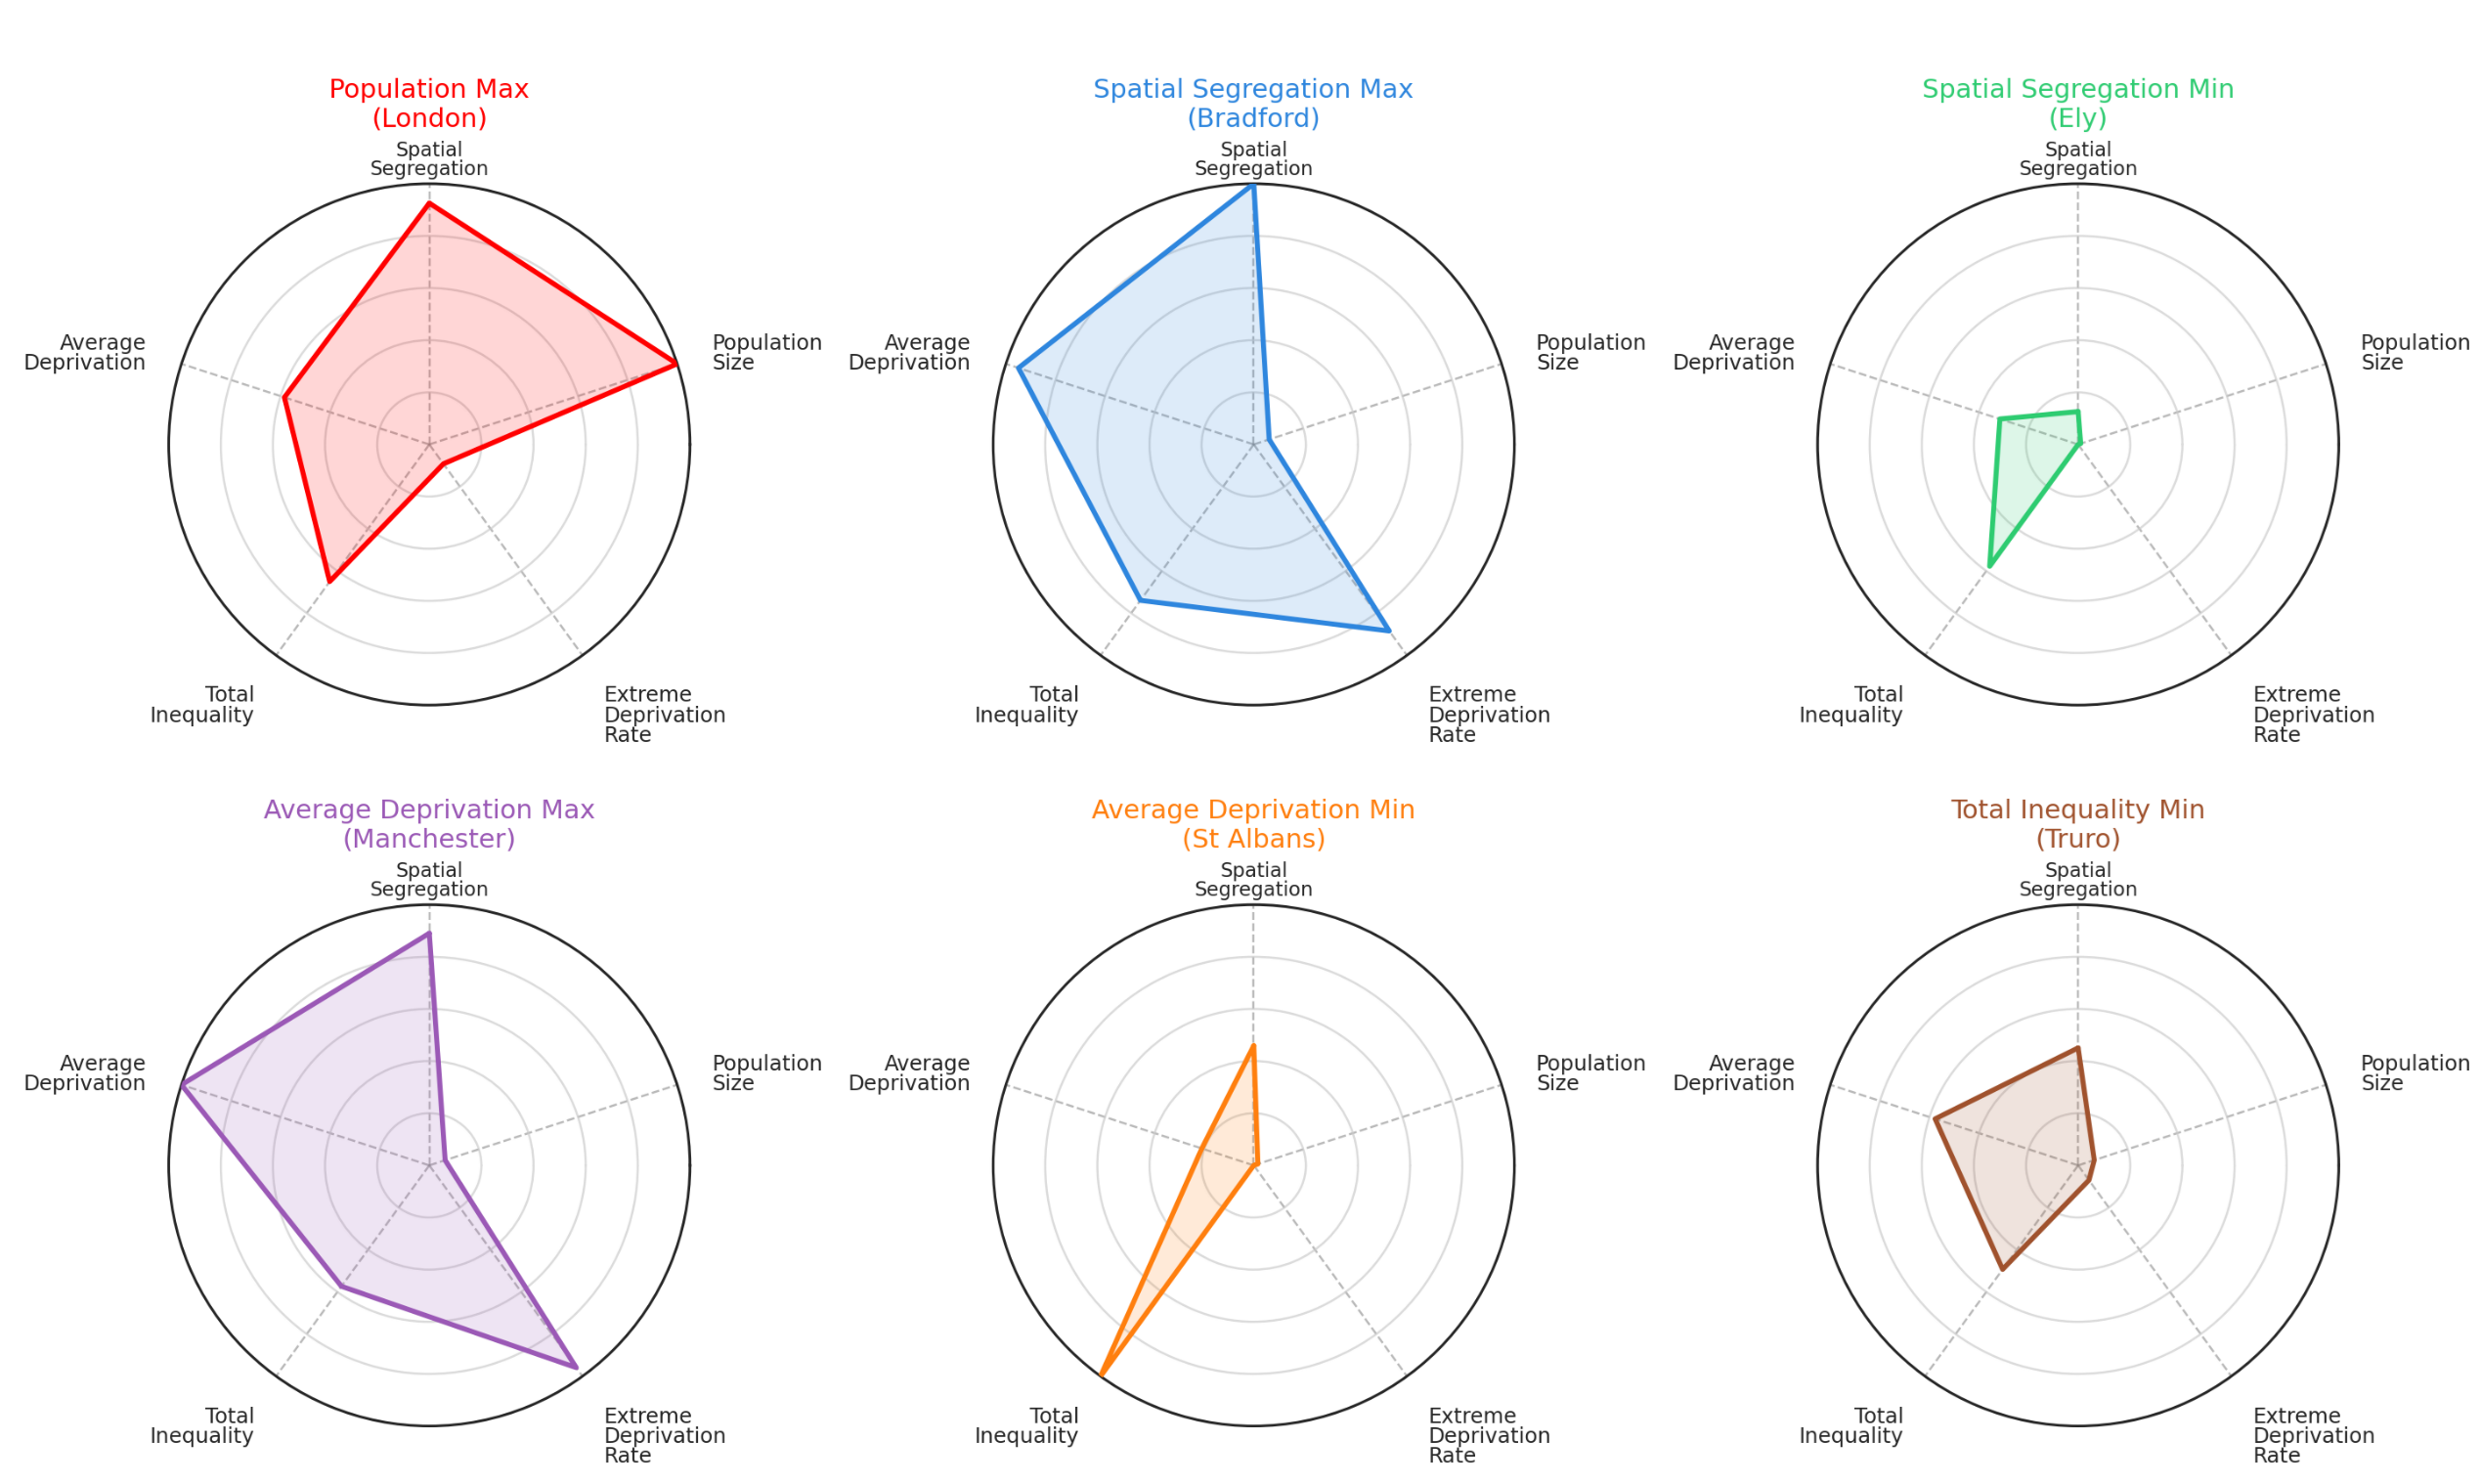
\includegraphics[width=0.9\textwidth]{figure3.png}
    \caption{Radar chart profiles of six extreme English cities across five distinct urban and deprivation indicators.}
    \label{fig:fig2}
\end{figure*}

\subsection{Aggregate Inequality Conceals Fundamentally Different Spatial Mechanisms}

Two cities with similar values of $G^*$ can differ sharply in their internal spatial structure. In one city the inequality may stem primarily from geographically contiguous clusters of deprivation, a pattern of systemic segregation, while in another it may arise mainly from localised mixing between neighbouring areas of different deprivation levels. $G^*$ as an aggregate measure cannot distinguish between these two mechanisms.

Figure 4 (Spatial vs Non-Spatial Inequality) ranks the full sample by $G^*$ and decomposes each city's inequality into its spatial component $G^*_S$ and non-spatial component $G^*_{NS}$. Among the ten most unequal cities, the most striking observation is not the ranking itself but the wide variation in the internal composition of inequality. St Albans and York have spatial shares $\gamma^*$ of only $38.2\%$ and $45.4\%$ respectively, meaning more than half of their internal inequality comes from the non-spatial component, reflecting deprivation differences that exist locally between adjacent neighbourhoods without forming geographically contiguous clusters. Leeds ($77.3\%$), Sheffield ($80.7\%$), and Newcastle ($78.0\%$) display the opposite pattern, with the large majority of their inequality driven by the geographic adjacency of high-deprivation neighbourhoods. The two groups occupy similar ranges of $G^*$ in absolute terms yet differ by more than 40 percentage points in spatial share.

\begin{figure}[t]
    \centering
    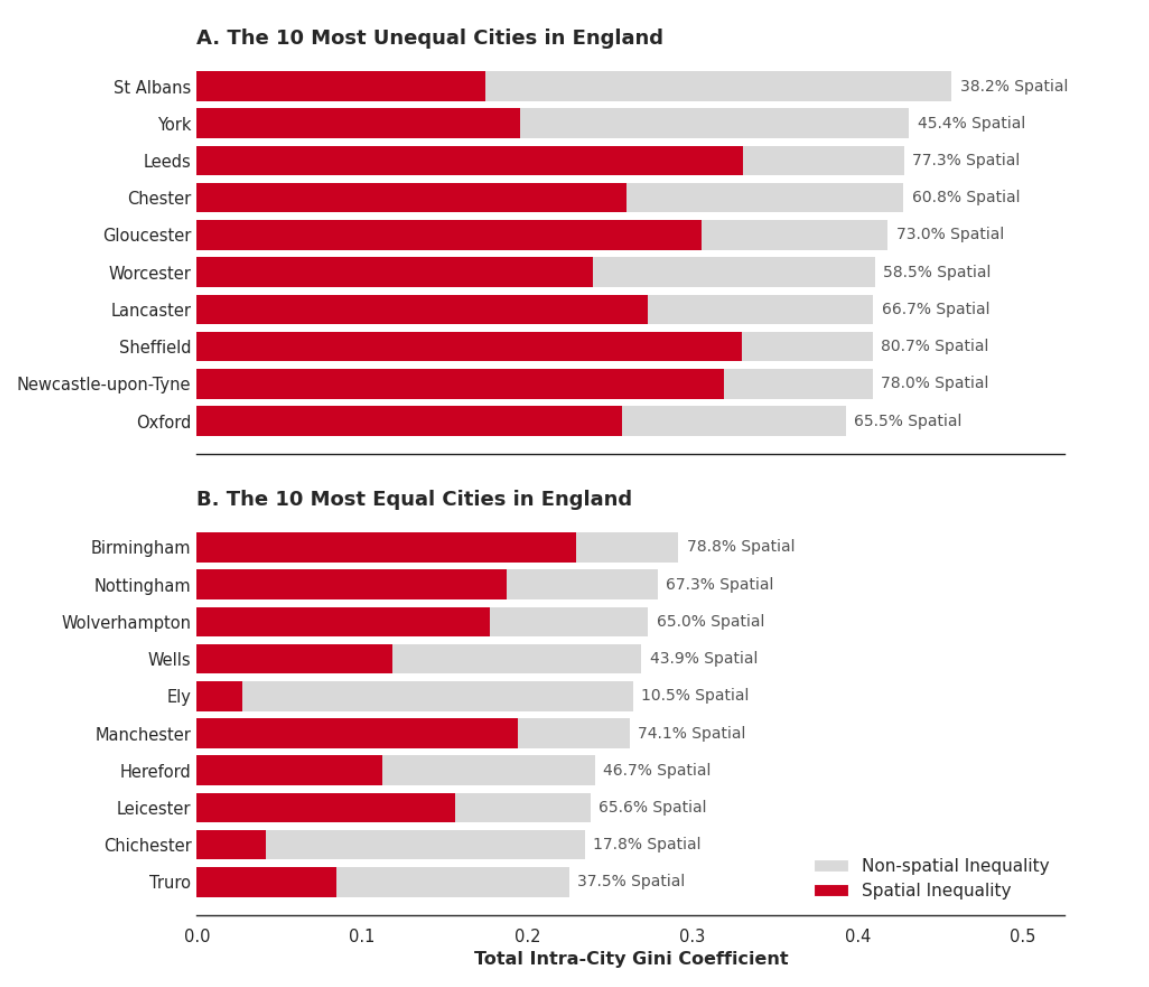
\includegraphics[width=1.0\columnwidth]{figure4.png}
    \caption{Spatial vs Non-Spatial Inequality}
    \label{fig:imd_structure}
\end{figure}

The same contrast appears among the ten most equal cities. Birmingham and Manchester have the highest $G^*$ values within that group but spatial shares of $78.8\%$ and $74.1\%$ respectively, showing that even relatively equal cities can exhibit highly spatialised inequality. Ely, by contrast, has both a very low $G^*$ and a spatial share of only $10.5\%$, representing a case of genuine internal homogeneity in which the inequality that does exist is neither large nor geographically concentrated.

The decomposition of the 15 largest cities (Figure 5) reinforces this pattern at the top of the urban hierarchy. London ($77.0\%$), Birmingham ($78.8\%$), Liverpool ($82.3\%$), and Bradford ($83.2\%$) all exceed $75\%$ in spatial share, suggesting that spatially organised deprivation inequality is the norm rather than the exception among England's largest cities.

\begin{figure}[t]
    \centering
    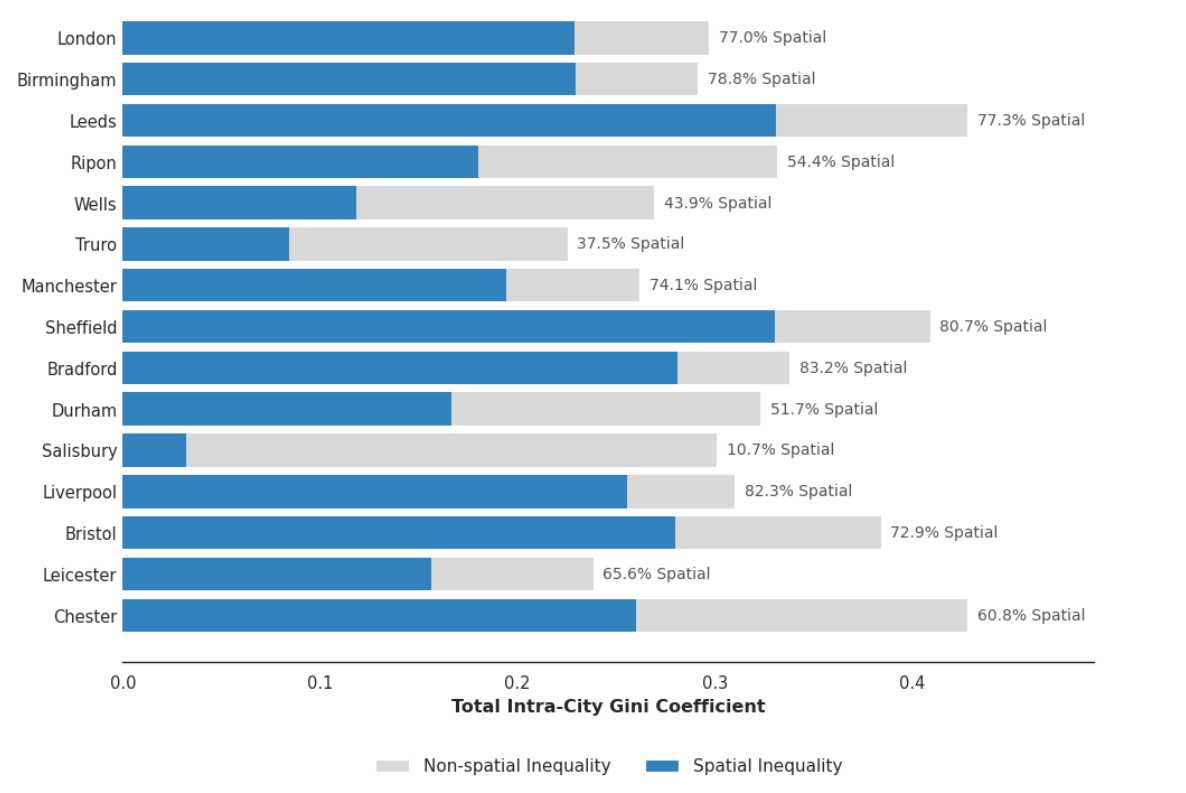
\includegraphics[width=1.0\columnwidth]{figure5.png}
    \caption{Inequality Decomposition in England's 15 Largest Cities}
    \label{fig:imd_structure}
\end{figure}

Taken together, these results establish that $G^*$ is a necessary but insufficient diagnostic tool. Two cities with the same $G^*$ but a 40 percentage point difference in spatial share face substantively different problems that call for different policy instruments.

\subsection{Systemic Segregation and Visible Neighbourhood Disparity Are Mechanistically Independent Forms of Inequality}

Having established that the spatial and non-spatial components differ in magnitude across cities, a natural question is whether they tend to co-occur. Do cities with high spatial segregation also tend to have high local neighbourhood disparity?

Figure 6 (Systemic Segregation vs Visible Neighbourhood Disparity) plots $G^*_S$ against $G^*_{NS}$ for all 54 cities. The distribution is highly scattered, the correlation between the two dimensions is weak, and all four quadrants are well populated. This pattern indicates that systemic spatial segregation and visible neighbourhood disparity are largely independent phenomena driven by different mechanisms.

\begin{figure}[t]
    \centering
    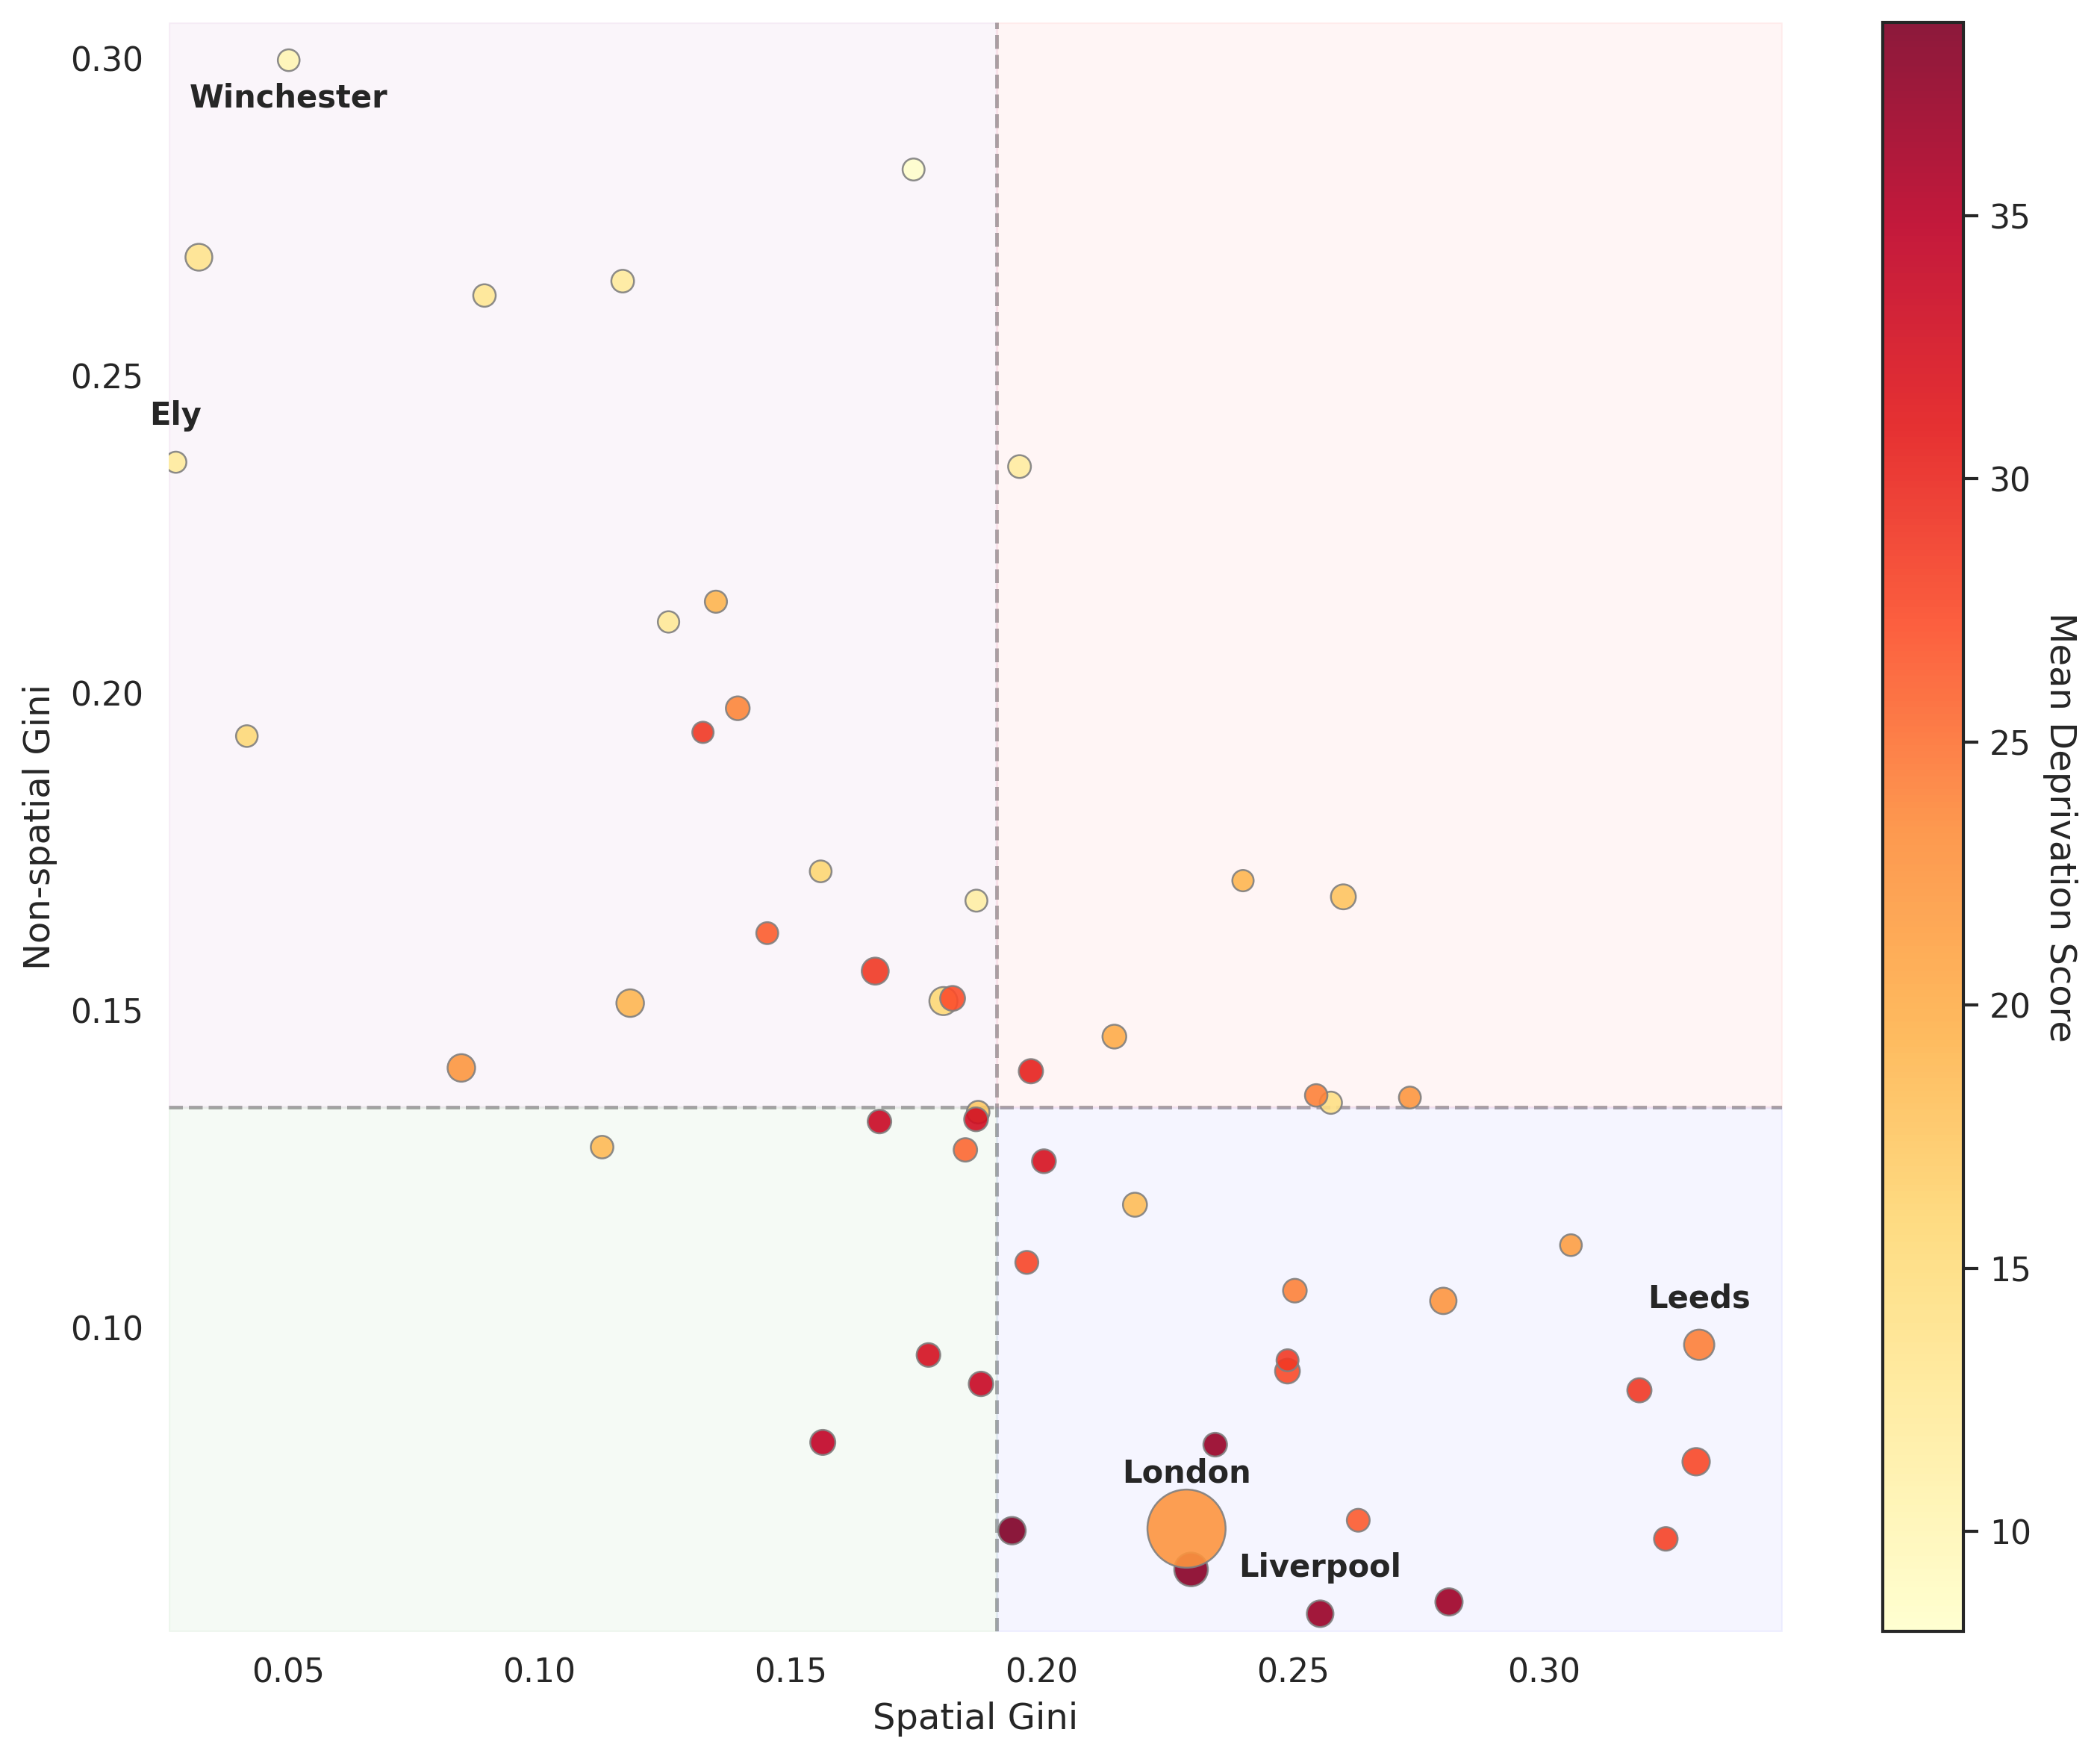
\includegraphics[width=1.0\columnwidth]{figure6.png}
    \caption{Systemic Segregation vs Visible Neighbourhood Disparity}
    \label{fig:imd_structure}
\end{figure}

The four quadrants correspond to meaningfully distinct urban types. Winchester and Ely, located in the upper-left quadrant with low $G^*_S$ and relatively high $G^*_{NS}$, exhibit deprivation differences that are genuine and perceptible at the level of adjacent streets, but these differences do not coalesce into contiguous deprived zones across the city. The inequality is fine-grained and locally visible. Leeds, London, and Liverpool, in the lower-right quadrant with high $G^*_S$ and low $G^*_{NS}$, present the opposite configuration: deprivation within any given neighbourhood is relatively uniform, but high-deprivation areas and low-deprivation areas are separated by large spatial distances at the city scale. This form of inequality is less perceptible at the street level yet constitutes a more deeply entrenched mechanism of geographic exclusion. Residents of high-deprivation clusters face not just a local shortage of resources but a structural disconnection from the opportunity landscape of the wider city. It is also notable that cities in this quadrant tend to have higher mean deprivation scores, which suggests a reinforcing relationship between systemic segregation and overall poverty.

The policy implication of this distinction is direct. Instruments designed to address visible neighbourhood disparity, such as targeted community investment and neighbourhood renewal programmes, are unlikely to be effective against systemic segregation, whose roots lie in city-scale patterns of residential sorting rather than in the resource allocation of any individual neighbourhood. Conflating the two mechanisms leads to policy effort being applied at the wrong geographic scale.

\subsection{City Size Is Systematically Associated with the Degree of Spatial Segregation}

As city population increases, the share of internal inequality attributable to systemic spatial segregation rises markedly, while the non-spatial component becomes progressively more dominant as city size decreases. This gradient is continuous across the full sample of 54 cities rather than a discrete categorical difference.

Figure 7 (The Demographic Transition of Inequality Components) plots $G^*_S$ and $G^*_{NS}$ as stacked contributions for all 54 cities ranked by population size. Among the 20 largest cities, $G^*_S$ is consistently high in absolute terms and accounts for a substantial share of $G^*$. From rank 21 onward, $G^*_S$ declines steadily, reaching very low levels among the 14 smallest cities, where $G^*_{NS}$ comes to dominate in relative terms. The transition from large to small cities takes the form of a smooth gradient in the chart rather than a step change.

\begin{figure}[t]
    \centering
    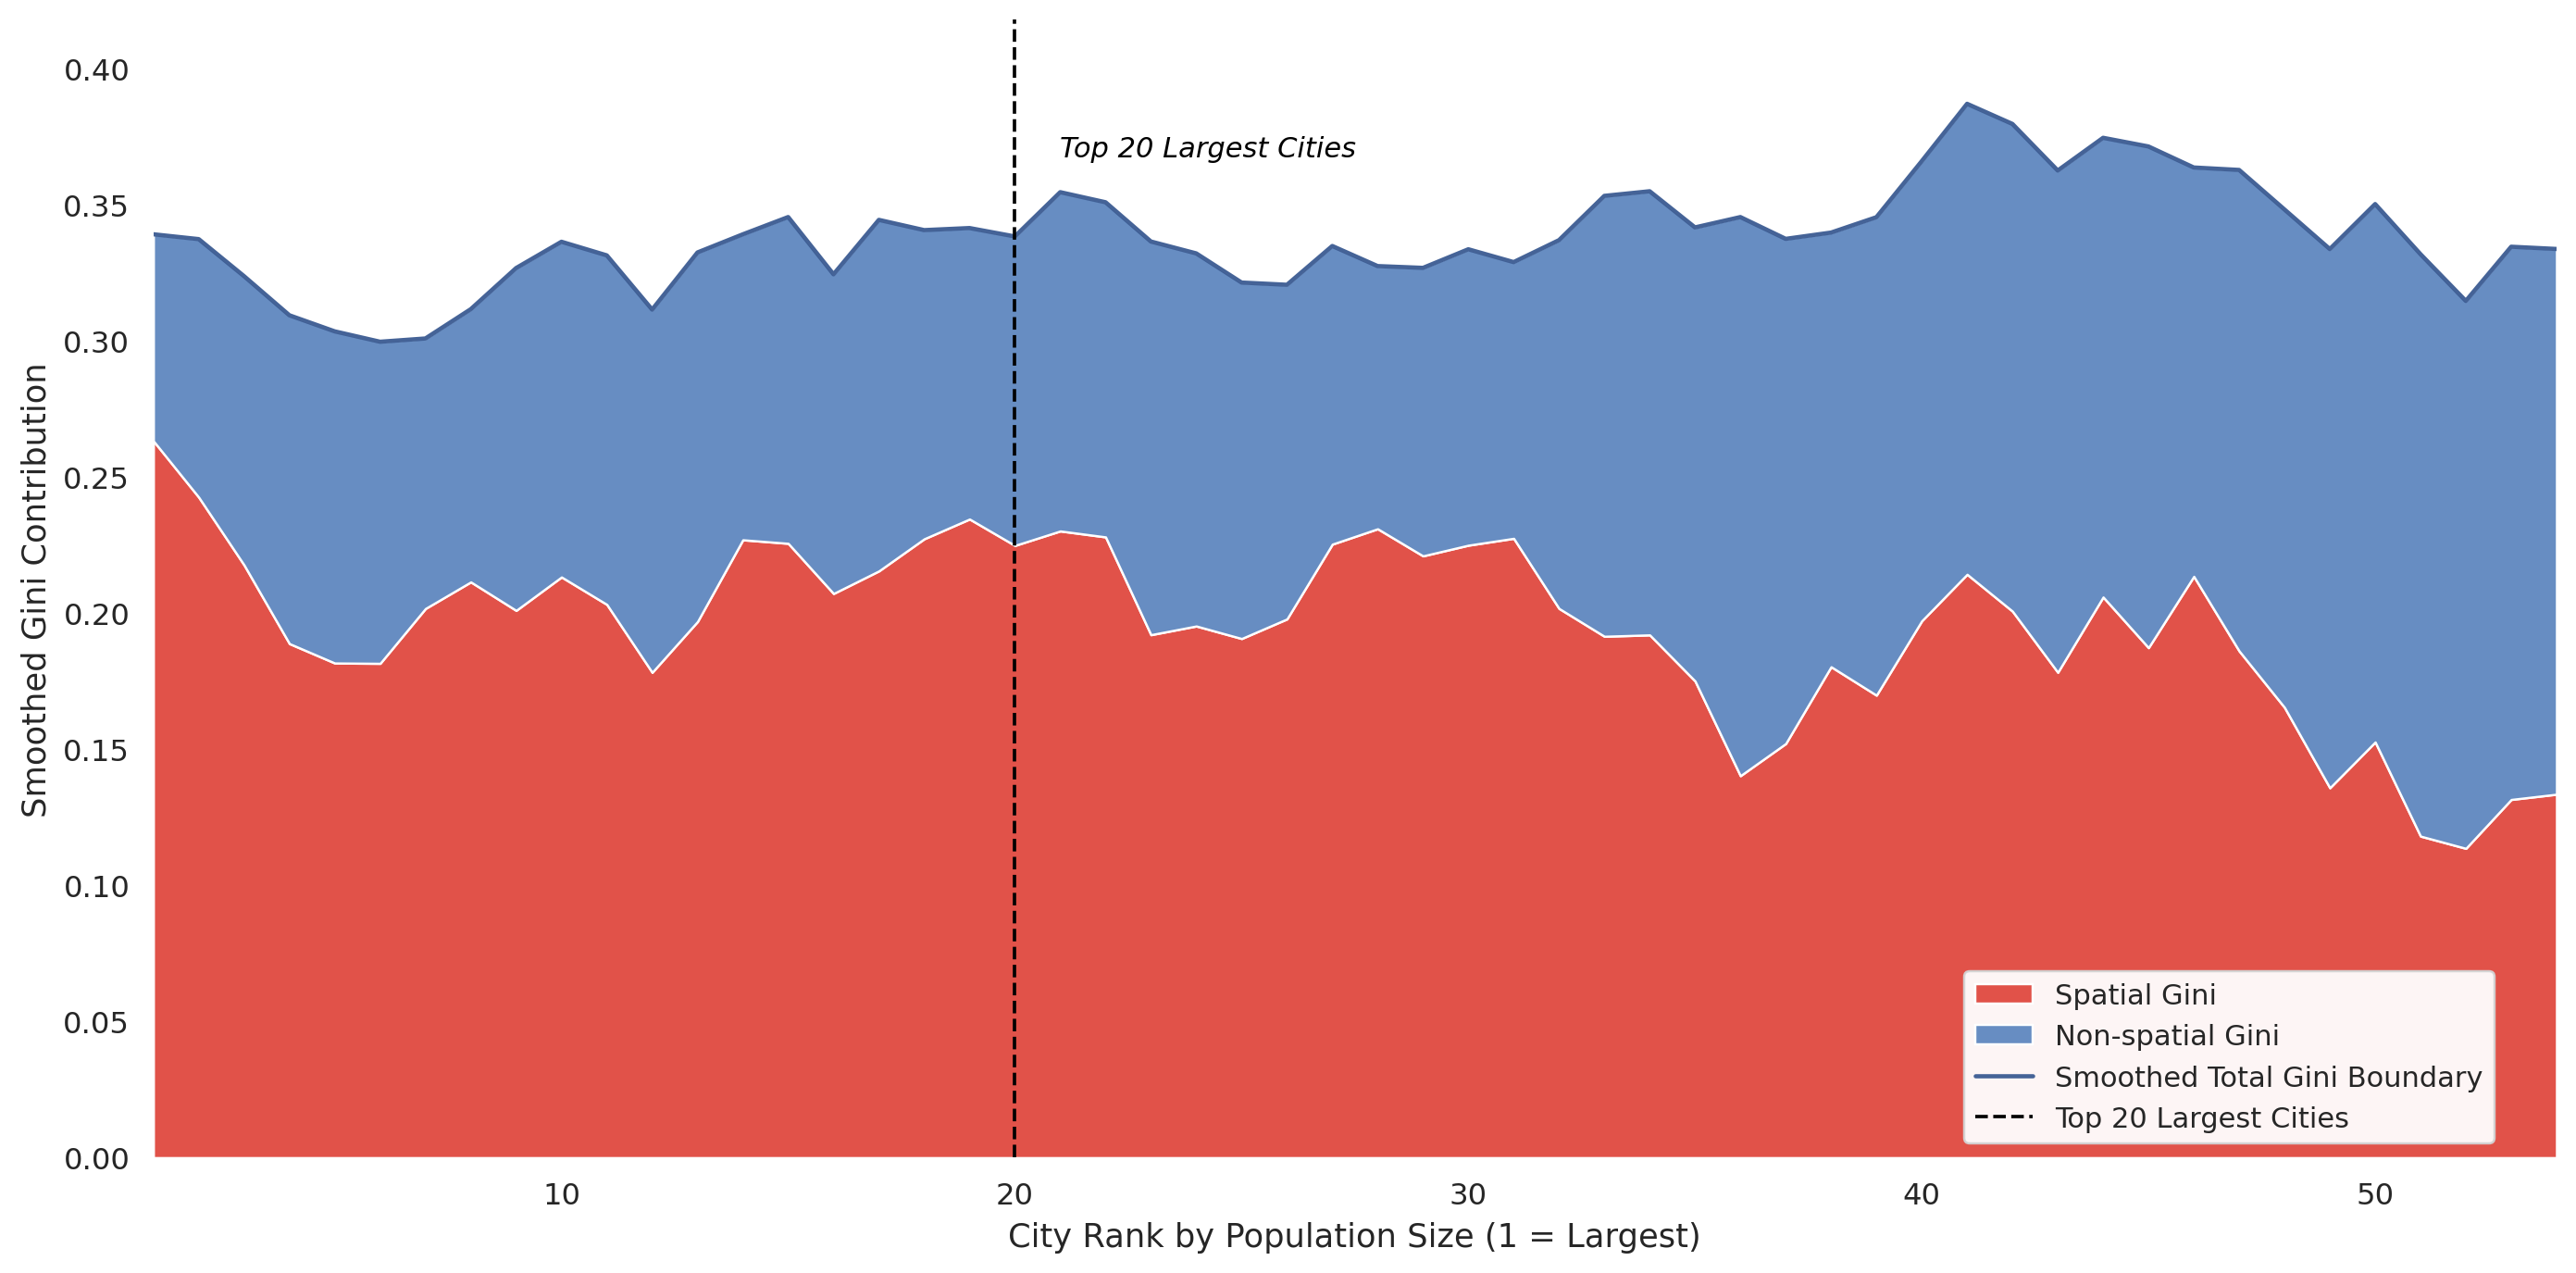
\includegraphics[width=1.0\columnwidth]{figure7.png}
    \caption{The Demographic Transition of Inequality Components}
    \label{fig:imd_structure}
\end{figure}

The decomposition of the 15 largest cities (Figure 5) provides complementary detail from the upper end of the size distribution. London, Birmingham, Leeds, Sheffield, and Liverpool all have $\gamma^*$ above $75\%$. Ripon ($\gamma^* = 54.4\%$), Durham ($\gamma^* = 51.7\%$), and Truro ($\gamma^* = 37.5\%$), which are the three smallest cities in the group of 15, have noticeably lower spatial shares, and their size ranks and spatial share ranks are highly consistent with each other.

Manchester is a notable departure from the overall pattern. As the seventh largest city in the sample, its $\gamma^*$ of $74.1\%$ sits at the lower end of the large-city range. This deviation is consistent with Manchester's broader profile of high mean deprivation and low $G^*$: when overall poverty is uniformly severe, the absolute deprivation gap between neighbourhoods is compressed, which in turn limits the scope for spatial differentiation. The Manchester case suggests that overall poverty level, not just city size, exerts an independent moderating influence on $\gamma^*$, a relationship that warrants systematic examination in future work.

The positive association between city size and spatial segregation is consistent with standard expectations from urban economics. Larger cities tend to have more pronounced labour market stratification, greater housing price differentiation, and more complex commuting cost structures, all of which encourage neighbourhoods of similar deprivation levels to cluster geographically. In policy terms, this implies that intervention strategies for large and small cities should operate at different geographic scales. For large cities, the priority is dismantling the structural patterns of residential segregation that span multiple neighbourhoods. For smaller cities, the challenge is closer to achieving fine-grained equity in the distribution of local community resources.


\bibliographystyle{abbrv}
\bibliography{ineqaulityref}

\end{document}
